\chapter{Background into Gamification}
	\label{chap:resources}
		
	% -- does gamification history need to go here? ---------  
	%The university has subscriptions to a vast number of major academic journals spanning a wide range of subject areas. By accessing the internet from a university network connection (Eduroam or Ethernet), the paywalls of many journals will simply vanish without any need for login credentials.

	\section{History of Gamification}
		
		Gamification is known as a powerful tool for engagement, which has, since its initial conception, now become a standard feature within software development \cite{history}. The term gamification first appeared in the context of software design in 2008 \cite{walz15}, but the term only started to get more widespread recognition within 2010. However, the term ‘‘gamification’’ was first coined by Nick Pelling in 2002 \cite{history}. Its initial aim was to incorporate the social and reward features of games into the software. Gamification started to gain much attention, so much so that it got described by a venture capitalist as one of the most promising areas of gaming \cite{wikigame}.
		
		Researchers consider gamification to be the progression of earlier work that focuses on adopting game-design elements to non-game situations and contexts. Research in the human-computer interaction field that uses game-driven elements for motivation and interface design suggests that there is a connection between Soviet concepts of socialist competition and the American management trend of ‘‘fun at work’’ \cite{wikigame}. 
		
		In 2010, Jane McGonigal delivered a groundbreaking TED Talk titled, ‘‘Gaming Can Make a Better World’ \cite{janeted}. This talk is considered the defining moment in the history of gamification. Within the talk, she prophesies a game based paradise. Where she states that “When I look forward to the next decade, I know two things for sure: that we can make any future we can imagine, and we can play any games we want, so I say: Let the world-changing games begin \cite{janeted}.” Hindsight informs she was right, as, from 2011, gamification starts to pick up steam. During this year, at a \ac{CHI} conference, a workshop titled “Gamification: Using Game Design Elements in Non-Gaming Contexts \cite{chi2011}”, which spawned the \ac{GRN} [11]. Through the years 2012 to 2016, gamification continues to grow. Even so, that gamification goes viral without people knowing through a game called Pokémon Go. Pokémon Go is one of the most successful applications of gamification with over 800 million downloads. People who would usually turn their nose up at badge collecting were out patrolling the streets searching for rare pokemon. Pokémon Go is one of the most successful apps of all time. It even broke records \cite{pokegwr,history}. It could be said thanks to Pokémon Go, that gamification is everywhere.
		
		Many established technology and other companies, including SAP AG, Microsoft, IBM, SAP, LiveOps, Deloitte, and other companies have started using gamification in various applications and processes \cite{silv11}.
		
		The increased popularity in gamification, within some contexts, has had led to many legal restrictions be placed upon it. However, this mainly refers to the use of virtual currencies and assets, as well as data privacy, data protection and labour laws. These laws are due to its nature of being a data mining systems that spread information online, known as data aggregator \cite{gamelaw,dataagg}.

	\section{The Science of Gamification}
		\label{sec:google_fu}
		
		Games are fun, and there is no denying that whether it is playing more traditional video games, mobile games or a recent phenomenon McDonalds Monopoly. The games industry is work an estimated \$2.3 trillion, showing that the global entertainment and media business is massive everywhere \cite{gamescience}. There is a reason behind this, as games made are crafted with the human brain in mind. From each roll of the dice, getting the correct combination, to defeating an opponent and enemy, to building a new settlement, each action rewards the brain, and its reward centre lights up \cite{sciencebehind}.
		
		By incorporating aspects from games like points, levels and progression bars into non-game situations, we can recreate the experience of gaming. Having these elements within a product, to interact with the user, is why gamification is so powerful.
		
		Games ranging from Super Mario Bros. to Monopoly have a real impact on brains and the way we learn. These impacts on are brain are due to dopamine. Dopamine is a neurotransmitter within a person’s brain that is triggered within a person whenever we do something positive or when a person feels that they have achieved something \cite{dopamine}. In essence, dopamine is a natural drug that makes people feel good \cite{sciencebehind}. This drug, dopamine, is an integral part of our learning through reinforcement learning. As Nestler Lab explains, “activation of the pathway tells the individual to repeat what it just did to get that reward \cite{sciencebehind, brainrewards}.” We do something well, and we get a sense of reward from our brains which leads us to do it again. Hence why we as humans tend to feel good when we are learning something; however, it is not very easy to stay motivated while learning as the learning requirements increases. At this stage is where gamification shines and can help keep the user/learner motivated with a little boost along the way. The motivation, the critical factor gamification tries to manipulate, is triggered by the sense of success. Which leads onto more willingness and desire to do something, this can be achieved by not only rewarding the final goal but by also releasing small amounts of dopamine as we are edging closer to a goal. Allowing a user to know if they are nearing a milestone can be achieved by using progress bars. Each sub-goal completed fills up the bar giving instant gratification, with small hits of satisfaction and dopamine, on the build-up to meeting the primary goal and that massive hit of dopamine, therefore creating that motivation to keep going. This situation becomes superseded only when an unexpected gratification situation occurs, releasing even more dopamine.
		
		While motivation is at the centre of gamification, our enthusiasm comes from three main areas: Autonomy; Value; Competence \cite{keepmotivation}. If someone is in charge of their destiny, they are more motivated to succeed. Allowing the person more control will mean that they will work harder towards objectives, especially for a more extended period, when given the opportunity and authority to select their direction when solving a problem. This aspect is giving them autonomy. The second principal area value is about the person feeling value to an activity or action. If the person feels that there is self-worth to the activity, then they will increase interest in the activity and increase their motivation levels. Research states that a positive correlation occurs when a student values a subject at school and their willingness to investigate a question. If the person cares, they will keep going and work harder until the task gets completed \cite{gamescience, keepmotivation}. Finally, the third area is competence. If a person develops a certain degree of proficiency at something, they are more likely to keep doing it. Another study has shown that there is a link between a student’s sense of mastery and their desire to continue certain activities. Those who give credit to natural talent rather than hard work will more likely give up more quickly.
		
		Gamification aims to take advantage of our extrinsic motivations, factors like final grades or money, and intrinsic motivation, traits like personal gains or enjoyment, to try and enhance our daily activities or tasks. Therefore, in order for the gamification to be most effective, then both these motivation factors need to be accounted for within the task. In order for the person to feel good about oneself, a form of reward has to exist \cite{gamescience}.
			
	\section{Gamification in Science}
		\label{sec:game_in_science}
		
		Although science concepts still use more conventional styles of gamification. Science concepts will often use a type of gamification game that has a primary purpose, which is other than just for pure fun, called a 'serious' or 'applied' game. These types of games get utilised by industries like scientific exploration, education, health care, defence, emergency management, city planning, engineering and politics \cite{wikiserious}. Although not all do, serious games tend to share aspects closely tied with simulational games. However, all serious games still have other gamification features included (see fig: \ref{fig:seriousg}).
		
		Nonetheless, in regards to the field of science, serious games' role is to include crucial activities for scientists. These include outreach, teaching and research. With serious games on the increase, an emerging sub-genre is called citizen science games (CSGs) \cite{10seriousrules}. CSGs enables the user to produce as well as, or instead, analyse data for scientific use. Some examples of CSGs are GalaxyZoo, Foldit and HiRE-RNA \cite{follett2015analysis,mazzanti2017can}
		
		\begin{figure}[t]
			\centering
			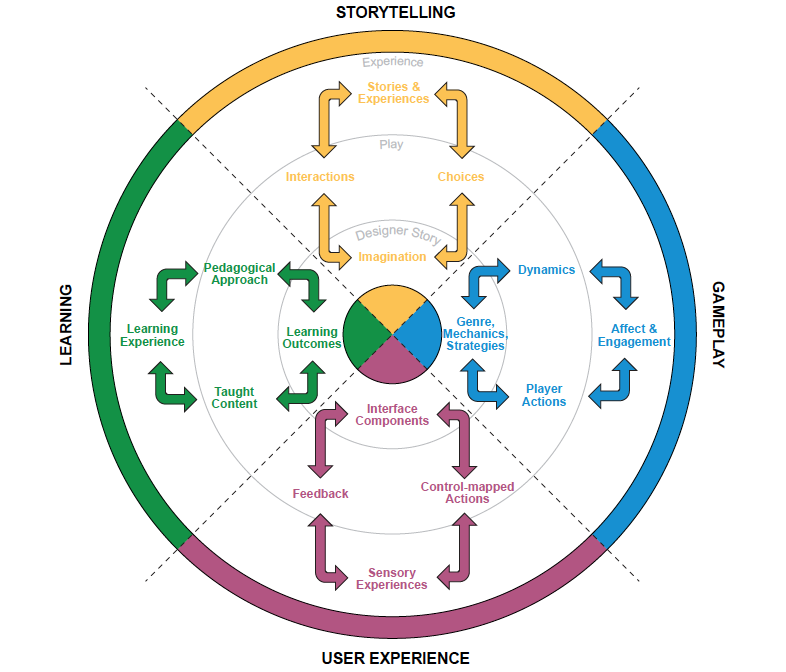
\includegraphics[height=6cm]{Serious-game-design-methodology}
			\caption{Serious game design methodology \cite{seriousmeth}}
			\label{fig:seriousg}
		\end{figure}
		
		Studies suggest that there are ten main rules for serious games to follow. These are \cite{10seriousrules}:
		\begin{enumerate}		
			\item Define a serious goal - we must first define the purpose of the game at the beginning of its development. Is its purpose for science, outreach, teaching or a combination of all three? 
			\item Get the balance between entertainment and serious tasks - the game design should be implemented as a function of the objectives of the game. Therefore equilibrium and compromise need to be found between scientific accuracy and player accessibility.
			\item Allow the player to interact with the scientific data - players interest increases if they can interact with the science data, enriching the learning experience. The ability for players to generate data also creates another perspective for the player, increasing interaction.
			\item Promote onboarding and engagement - Expectations of players are varied. Therefore the reward system needs to be versatile. Ideally, the entry-level should be low and the difficulty altered to each player.
			\item Manage Information Flow - How the information to the play gets received will impact their behaviour, either positively or negatively. So if the focusing is on the outcome, this could influence the results.
			\item Provide an appropriate narrative - This is important for all games, but also crucial for serious games. The narrative should give the player context to the game, allowing them to know what to do. 
			\item Adapt the level design - Depending on the objective, variation on level designs needs implementing. These can include duration, tasks and difficulty. 
			\item Develop good graphics that are not just pleasing on the eye - High-quality graphics increase the player's immersion into the game.
			\item Use all modalities, especially sound - Using just a visual channel can overload the player. Therefore it is vital to take the load of the player's vision and use several different channels — for example, sound.
			\item Iteratively assess what works and what does not - However, it is vital to take into account three different perspectives for serious games. The developer, the player and the scientist as they all have different views on what they believe the game needs adapting based on their desires.
		\end{enumerate}
	
	\section{Gamification in Education}
		\label{sec:gamification_edu}
		
		The gamification of learning is an educational approach to motivate students to learn by using game elements in a learning environment \cite{gamelearning}. Which is very much the same thing as gamification in general, but more of a focus on learning. However, gamification in learning has two main views within academia. One that categories gamification of learning as learning, with game-like features, but only when learning is happening in a non-game context, like a classroom. This version would involve a range of elements that get presented in a system, or game layer, which aims to happen in parallel to the learning in a regular classroom. At the same time, the other half includes games that have been designed to induced learning within them \cite{gamelearning} (see fig: \ref{fig:badges}).
		
		\begin{figure}[t]
			\centering
			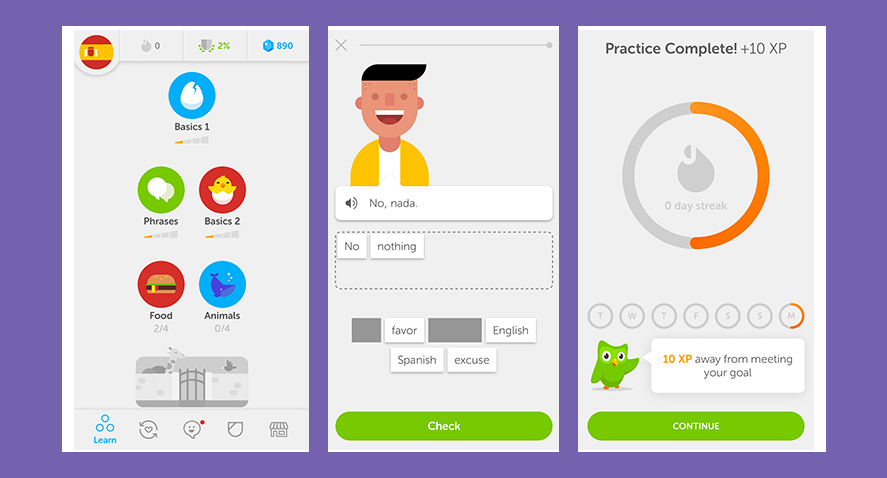
\includegraphics[height=5cm]{gamification2}
			\caption{Example of gamification in action \cite{edugamexample}}
			\label{fig:badges}
		\end{figure}
		
		Gamification within an educational or learning situation has multiple benefits. It is not just about trying to improve attendance with incentives by reaching a particular score, or extra rewards for completing specific tasks within a lesson. It can aid in cognitive development in adolescents, increase levels of engagement and can aid with accessibility within the classroom \cite{5benefits}. Games produced for enhancing cognitive development are known as "brain games" \cite{5benefits}. These popular games typically are centred around a series of questions and problems for the player to solve or answer. These games improve the rate the player can maintain information and increase the brain's ability to process information. The levels of engagement increase, when gamification has been used, within a classroom. A study was performed by scientists, which aimed to measure students levels of engagement in a classroom where gamification elements where are used \cite{eduengage}. They assigned a point system to multiple daily activities. Each student had a measurement of the perceived level of engagement. Its finding is that the game like setting was supporting the learning within the classroom and increased productivity. By increasing engagement levels, it also means it helps students be able to access the content of the lesson, that is or needs to be delivered. 
		
		Even though gamification can aid teaching students of all needs, a study conducted on students who had autism using video games showed that this training package was powerful in teaching content that was age-appropriate \cite{autismedu}. However, gamification of learning is not something just for the classroom; its an excellent tool for learning outside the classroom. Games like Spore create a deeper understanding of life and evolution as the game simulates a world where the player's character will evolve, adapting to their surroundings through reproduction. Another game by the same creator, Will Wright, Sim City aims to teach the player key skills like \cite{simfact}: Supply and demand; Budgeting; Urban planning; Managing the environment; Understanding utilities and services like transport systems and public services; Reading and maths skills.
		
		Gamification of learning has excellent potential benefits. The benefits involve \cite{gamelearning}: Allowing students to have ownership of their learning, as well as giving opportunities for the learner to gain a sense of their 'own identity', through alternative role-playing selves. The freedom, without any negative repercussions, to fail and keep on trying again. The ability to increase fun and joy while learning. The opportunity for tasks to be differentiated. Making the learning visible and providing opportunities to inspire intrinsic motivators for learning. Also, the ability to aiding in motivating students with low levels of motivation.